\capitulo{Elementos de geometr\'ia diferencial}{}
%{Pedro Walter Lamberti}

\begin{epigrafe}
  $\acute{\alpha}    \gamma\epsilon     \omega    \mu    \acute{\epsilon}    \mu
  \acute{\epsilon} \tau \rho \eta \tau o \varsigma \;\; \mu \eta \delta
  \epsilon \iota \varsigma \;\; \epsilon \iota \sigma \iota \tau \omega$  \\
  Que  no ingrese  nadie  que no  sepa geometr\'ia.   \autortituloepigrafe{Frase
    grabada en la entrada de la Academia de Plat\'on}
\end{epigrafe}


% =============================== Introduccion =============================== %

\seccion{Estructuras}
\label{s:WL:Introduccion}

Una  de  las  nociones m\'as  elementales  de  la  matem\'atica  es la  de  {\it
  conjunto}.   Un  conjunto  es   una  colecci\'on  de  elementos  perfectamente
caracterizados.   Los  elementos  pueden   ser  de  cualquier  tipo:  n\'umeros,
funciones, personas, autos, etc. El  enfoque matem\'atico moderno es ir montando
estructuras de  distinta naturaleza sobre  un dado conjunto. En  este cap\'itulo
comenzaremos con la noci\'on de espacio topol\'ogico y llegaremos al concepto de
variedad Riemanniana. Este procedimiento ha mostrado ser de utilidad en el marco
de la f\'isica, que es nuestro principal \'ambito de inter\'es.  El mapa de ruta
de las distintas estructuras que veremos en este cap\'itulo es el siguiente:
%
\begin{itemize}
\item Espacio topol\'ogico (continuidad)
\item Espacio m\'etrico (distancia)
\item Variedad topol\'ogica (coordenadas)
\item Variedad diferenciable (diferenciabilidad)
\item Estructura afin (paralelismo)
\item Estructura m\'etrica (Finsler y Riemann)
\end{itemize}

Si  bien   existe  una  estructura   intermedia  entre  la  topol\'ogica   y  la
diferenciable,  que se  conoce como  {\it  estructura lineal  a trozos},  aqu\'i
prescindiremos de su estudio. A  su vez, hay otras estructuras matem\'aticas que
son usadas en el marco de  las teor\'ias f\'isicas. Se destacan la estructura de
producto  interno sobre  un espacio  vectorial complejo,  la cual  conduce  a la
noci\'on  de  espacio  de  Hilbert,  de fundamental  importancia  en  mec\'anica
cu\'antica;  la estructura simpl\'ectica,  \'util en  mec\'anica cl\'asica  y la
estructura de K\"ahler, de relevancia en teor\'ia de cuerdas.

% ============================ Espacio Topologico ============================ %

%Comenzaremos con la noci\'on de espacio topol\'ogico.
%\sub
\seccion{Espacio Topol\'ogico}
\label{s:WL:EspacioTopologico}

Un conjunto  arbitrario $X$  est\'a desprovisto de  toda estructura  que permita
definir nociones tales como la {\it convergencia} de una sucesi\'on de elementos
de  $X$, la  {\it proximidad}  de dos  elementos de  $X$, etc.  En  principio se
dispone s\'olo de las operaciones  elementales de {\it uni\'on} $\bigcup$ e {\it
  intersecci\'on} $\bigcap$ de  subconjuntos. Estas operaciones tambi\'en pueden
realizarse entre  distintos conjuntos.  Denotaremos con $\emptyset$  al conjunto
vac\'io. Surge entonces el desaf\'io de construir alguna estructura matem\'atica
definida  sobre $X$  que  permita definir,  de  manera precisa  las nociones  de
proximidad, continuidad, convergencia, etc. Esto  se logra a trav\'es de la idea
de una {\bf topolog\'ia} sobre $X$.

\begin{definicion}[Topolog\'ia]
  Una  {\it topolog\'ia}  $\Upsilon$ sobre  el conjunto  $X$ es  una  familia de
  subconjuntos de $X$ que cumple con las siguientes condiciones:
  %
  \begin{enumerate}
  \item $X$ y $\emptyset$ est\'an en $\Upsilon$: $X, \emptyset \in \Upsilon$
  %
  \item  La  intersecci\'on de  cualquier  colecci\'on  finita  de elementos  de
    $\Upsilon$ est\'a en $\Upsilon$:
    \[
    A_i \in  \Upsilon, \quad \forall  \: i  = 1 ,  \ldots , n  \quad \Rightarrow
    \quad \bigcap_{i=1}^n A_i \in \Upsilon
    \]
  %
  \item La uni\'on de una colecci\'on arbitraria --finita o no-- de elementos de
    $\Upsilon$, pertenece a $\Upsilon$:
    \[
    A_i \in \Upsilon \quad \Rightarrow \quad \bigcup_i A_i \in \Upsilon
    \]
  \end{enumerate}
\end{definicion}

\begin{definicion}[Espacio topol\'ogico y abiertos]
  Al par $(X,\Upsilon)$ lo  llamaremos {\it espacio topol\'ogico}. Los conjuntos
  que est\'an en $\Upsilon$ se llaman {\it abiertos}.
\end{definicion}


%{\it 
Ejemplos:
%}:
%
\begin{itemize}
\item {\it  Topolog\'ia trivial}. Es la  que consta de s\'olo  dos elementos, el
  conjunto vac\'io y el conjunto total $X: \Upsilon = \{ \emptyset , X \}$.
%
\item {\it Topolog\'ia discreta}. Es la que en todo subconjunto de $X$ est\'a en
  $\Upsilon$, es decir $\Upsilon =  \P(X)$ donde $\P(X)$ representa a las partes
  de $X$.
%
\item En  los cursos elementales  de an\'alisis matem\'atico hemos  estudiado en
  $\Rset^n$, es decir el conjunto de $n$-tuplas de n\'umeros reales, la noci\'on
  de bolas abiertas. M\'as precisamente,  una bola abierta en $\Rset^n$ centrada
  en el punto $p = (p_1,...,p_n) \in \Rset^n$ y de radio $r > 0$ es el conjunto
  \[
  \B_{r,p} = \left\{ (x_1 , \ldots , x_n) \in \Rset^n:   \: 0 \le   \sqrt{\sum_i
      (x_i-p_i)^2} < r \right\}
  % \text{tal que} \;\; 0\leq \sqrt{\sum_i (x_i-p_i)^2}<r}
  \]
  %
  La  colecci\'on de  todas  las  bolas abiertas  en  $\Rset^n$ constituyen  una
  topolog\'ia  para $\Rset^n$.   Se conoce  como la  {\it topolog\'ia  usual} de
  $\Rset^n$.\newline Obs\'ervese que un  subconjunto $A$ de $\Rset^n$ es abierto
  (en el sentido  usual), cuando para todo  $x \in A$, existe un  $\varepsilon > 0$
  tal que $\B_{\varepsilon,x} \subset A$.
\end{itemize}

\begin{definicion}[Entorno]
  Un {\it entorno} de un punto $x \in X$ es un conjunto $U$ que contiene a $x$ y
  tal que existe un  abierto $V$ contenido en $U$: $x \in  V \subseteq U$ con $V
  \in \Upsilon$.
\end{definicion}

\begin{definicion}[Funci\'on continua]
  Sea $f: X  \rightarrow Y$ una funci\'on entre  dos espacios topol\'ogicos $(X,
  \Upsilon)$ e  $(Y,\omega)$. $f$ es una  {\bf funci\'on continua} en  $x \in X$
  sii dado cualquier entorno abierto $U  \subset Y$ de $f(x)$, existe un entorno
  de $x$,  $V \subset  X$ tal  que $f(V) \subset  U$. Equivalentemente  se puede
  definir  una  funci\'on continua  de  la siguiente  manera:  $f$  es una  {\it
    funci\'on continua}  sii la  imagen inversa de  cada conjunto abierto  es un
  abierto.
\end{definicion}
%
%Equivalentemente se puede definir una funci\'on continua de la siguiente manera:
%
%\begin{definicion}[Funci\'on continua]
%  Sea $f: X \rightarrow Y$  una funci\'on entre dos espacios topol\'ogicos $(X,
%  \Upsilon)$ e $(Y,\omega)$. $f$ es  una {\bf funci\'on continua} sii la imagen
%  inversa de cada conjunto abierto es un abierto.
%\end{definicion}
Es f\'acil demostrar la equivalencia entre ambas definiciones, y hacerlo queda como ejercicio para el lector.

\begin{definicion}[Homomorfismo]
  Un {\it homomorfismo} $\Psi$ entre dos espacios topol\'ogicos $(X,\Upsilon)$ e
  $(Y,\omega)$ es una funci\'on $\Psi: X \rightarrow V \subseteq Y$
  %
  % \[
  % \Psi: X \rightarrow V \subseteq Y
  % \]
  biyectiva, continua y con inversa continua.
\end{definicion}

\begin{definicion}[Sucesi\'on]
  Una  {\it  sucesi\'on}  en un  conjunto  $X$  es  una aplicaci\'on  $s:  \Nset
  \rightarrow   X$   donde   $\Nset$   es   el   conjunto   de   los   n\'umeros
  naturales. Denotaremos a la sucesi\'on por $\{ x_n \}_{n \in \Nset}$.
  % \text{donde } n \in \Nset$
\end{definicion}

En un espacio topol\'ogico podemos introducir la noci\'on de convergencia de una
sucesi\'on. Obs\'ervese  que \'esto  es posible gracias  a que disponemos  de la
noci\'on de conjunto abierto.

\begin{definicion}[L\'imite]
  Sea $(X,  \Upsilon)$ un espacio topol\'ogico  y $\{ x_n \}_{n  \in \Nset}$ una
  sucesi\'on en $X$. Diremos que $x$ es  el {\it l\'imite} de $x_n$ si para todo
  entorno $V$ de $x$,  existe un $n_0 \in \Nset$ tal que  $\forall n \ge n_0$ se
  tiene que $x_n \in V$.
\end{definicion}

Los l\'imites de  las sucesiones no tienen porque  ser \'unicos. Una condici\'on
que debe cumplir el espacio  topol\'ogico $(X,\Upsilon)$ para que las sucesiones
tengan un \'unico l\'imite es que  dados dos puntos distintos $x \ne y$,con $x,y
\in X$ existen entornos disjuntos de $x$ e $y$. A los espacios topol\'ogicos que
cumplen  con esta  condici\'on se  los llama  espacios de  Hausdorff  o espacios
$T_2$.


% ============================== Espacio Metrico ============================= %

%\sub
\seccion{Espacios m\'etricos}
\label{s:WL:Metrico}

En el  tercer ejemplo de espacio  topol\'ogico, usamos la  noci\'on de m\'etrica
eucl\'idea  para definir las  bolas abiertas  en $\Rset^n$.  El disponer  de una
m\'etrica  no es  algo que  ocurre  en todo  conjunto. Eso  motiva la  siguiente
definici\'on:
%
\begin{definicion}[Espacio m\'etrico]
  Un {\it  espacio m\'etrico} en un conjunto  $X$ munido de una  funci\'on $d: X
  \times X \rightarrow \Rset_+$ tal que se cumplen las condiciones:
%
\begin{enumerate}
\item $d(x,y) \ge 0 \quad \forall \: x , y \in X$ y la igualdad se cumple sii $x
  = y$,
%
\item\label{Metrica:simetria} $d(x,y) = d(y,x)$ \ simetr\'ia.
%
\item\label{Metrica:triangular} $d(x,y) \le d(x,z) +  d(z,y) \quad \forall x , y
  , z \in X$.
\end{enumerate}
\end{definicion}
%
\noindent   La   \'ultima   condici\'on   se  conoce   como   {\it   desigualdad
  triangular}.  Mas adelante  en este  libro veremos  funciones $d:  X  \times X
\rightarrow \Rset_+$ que  no satisfacen ni la condici\'on~\ref{Metrica:simetria}
ni  la condici\'on~\ref{Metrica:triangular},  pero que  sin embargo  sirven para
medir cu\'an separados est\'an dos puntos de $X$. En ese caso diremos que $d$ es
una {\it distancia} definida sobre $X$.%%% ??? DIVERGENCIA?


% ============================ Variedad Topologica =========================== %

%\sub
\seccion{Variedad Topol\'ogica}
\label{s:WL:VariedadToplogica}

Nuestra experiencia cotidiana de percibir  que estamos inmersos en un espacio de
3 dimensiones, en el cual  podemos medir \'angulos y determinar distancias entre
dos puntos, ha  hecho que usemos estas caracteristicas  de nuestro habitat, como
motivaci\'on de  la defici\'on de ciertas estructuras  matem\'aticas en espacios
abstractos.

En primer lugar, con la noci\'on de una variedad topol\'ogica buscaremos simular
en  un conjunto  cualquiera, la  noci\'on  de cercan\'ia  y dimensionalidad  que
tenemos en $\Rset^n$.

\begin{definicion}[Variedad topol\'ogica $n$-dimensional]
  Una  {\it Variedad  topol\'ogica $n$-dimensional}  es un  espacio topol\'ogico
  $\M$ tal que es {\it localmente eucl\'ideo}, es decir que para cada $x \in \M$
  existe  un  entorno  abierto $U$  de  $x$,  homeomorfo  a  un abierto  $V$  de
  $\Rset^n$: \ $\phi: U \subseteq \M \rightarrow \Rset^n$ \
  %
  % \[
  % \phi: U \subseteq \M \rightarrow \Rset^n
  % \]
  %
  tal que \ $\phi:U \rightarrow V$ \
  % \[
  % \phi:U \rightarrow V
  % \]
  y  $\phi$ es  un homeomorfismo.  Tambi\'en  pediremos que  $\M$, como  espacio
  topol\'ogico, sea un espacio Hausdorff.
\end{definicion}
%
A los pares  $(U,\phi)$ se los denominan {\it cartas sobre  $\M$}. Se supone que
la  colecci\'on de  todas las  cartas cubren  completamente a  $\M$.  Las cartas
permiten asignar {\it coordenadas} a $\M$:
%
\[
\mbox{Si}  \quad  p \in  U  \subseteq \M  \quad  \mbox{entonces}  \quad \phi:  p
\rightarrow (p_1 , \ldots , p_n) \in \Rset^n
\]

\begin{figure}[h!]
  \centerline{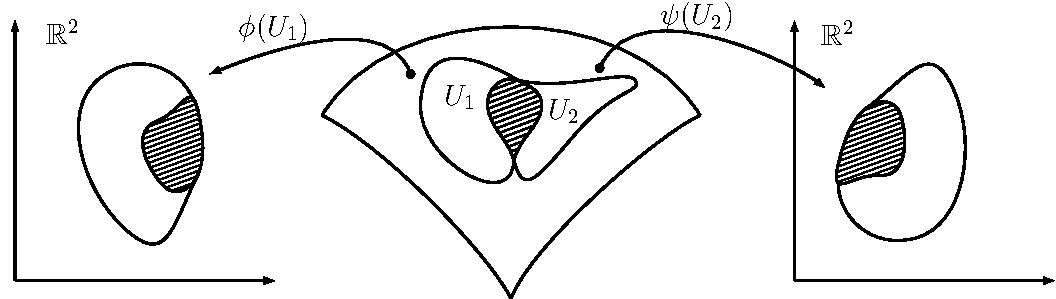
\includegraphics[width=13cm]{figura1.pdf}}          \leyenda{Cartas
    coordenadas usadas en la definici\'on de una variedad topol\'ogica.}
\end{figure}

A  la colecci\'on  de n\'umeros  reales $(p_1  , \ldots  , p_n)$  se  llaman las
coordenadas  de  $p$  de  acuerdo  a  la carta  $(U,\phi)$.   La  existencia  de
coordenadas, es el aspecto fundamental por el que el concepto de variedad es tan
\'util en f\'isica.

Podr\'ia suceder que un mismo punto $p$ pertenezca a m\'as de una carta, digamos
$(U_1,\phi_1)$  y  $(U_2,\psi_2)$.  En  ese  caso  hablaremos  de un  cambio  de
coordenadas:
%
\begin{equation}\label{cc}
\psi \circ \phi^{-1}: \phi(U_1 \cap U_2) \rightarrow \psi(U_1 \cap U_2)
\end{equation}
%
Si denotamos por $(p_1 , \ldots  , p_n)$ a las coordenadas correspondientes a la
carta  $(U_1,\phi_1)$  y  por  $(\tilde{p}_1  , \ldots  ,  \tilde{p}_n)$  a  las
correspondientes a la carta  $(U_2,\psi_2)$, entonces las funciones $\tilde{p}_i
= \tilde{p}_i(p_1 ,  \ldots , p_n)$ son funciones continuas, y  dan el cambio de
coordenadas. Estas funciones son invertibles con inversa continua.

Ejemplos de variedades topol\'ogicas son:
%
\begin{itemize}
\item $\Rset^n$. En este caso hay  una carta coordenada global que cubre toda la
  variedad y donde el homeomorfismo es la identidad.
%
\item $\Sset^n$, la esfera de dimensi\'on $n$. Ella est\'a definida como el conjunto:
  \[
  \Sset^n = \left\{  (x_1 , \ldots ,  x_{n+1}), \: x_i \in \Rset:  \quad x_1^2 +
    \cdots + x_{n+1}^2 = 1 \right\}
  % \text{ tales que }
  \]
\end{itemize}
%
\noindent  Se debe observar  que al  definir $\Sset^n$  no estamos  pensando que
est\'a inmersa  en $\Rset^n$. En este  caso podemos usar  las siguientes cartas:
$(U_N,  \phi_N)$ y $(U_S,\phi_S)$,  donde $U_N  = \Sset^n-\{  (0,0,\ldots,1) \},
\quad U_S = \Sset^n -{(1,0,\ldots,0)}$ y los mapas
%
\[
\phi_N:  U_N  \rightarrow  \Rset^n  /  (\phi_N(x_1  ,  \ldots  ,  n_{n+1}))_i  =
\frac{x_i}{1-x_{n+1}}
\]
%
y
%
\[
\phi_S:  U_S  \rightarrow  \Rset^n  /  (\phi_N(x_1  ,  \ldots  ,  n_{n+1}))_i  =
\frac{x_i}{1+x_{n+1}}
\]
%
Ambos mapas son homeomorfismos.  Observemos  que $\phi_N(x_1 , \ldots , x_{n+1})
= (t x_1 , \ldots , t x_n)$ y  $\phi_S(x_1 , \ldots , x_{n+1}) = (u x_1 , \ldots
,  u  x_n)$   con  $t  =  \frac{1}{1-x_{n+1}}$  y   $u  =  \frac{1}{1+x_{n+1}}$,
respectivamente.  Es directo verificar la  inyectividad pues si $(t x_1 , \ldots
, t x_n) = (t  y_1 , \ldots , t y_n) \Rightarrow x_i =  y_i \quad \forall \: i$.
Entonces  los puntos  $x$  e $y$  son  id\'enticos.  Para  ver la  suryectividad
consideremos el punto  $y = (y_1 , \ldots  , y_n) \in \Rset^n$. Si  tomamos $x =
\left( t^{-1}  y_1 ,  \ldots , t^{-1}  y_n ,  y_{n+1} \right)$ con  $t \ne  0$ e
$y_{n+1} =  t \sqrt{1-(t^{-1}  y_1)^2 - \cdots  - \left( t^{-1}  y_n \right)^2}$
vemos que para cada $y \in \Rset^n$ existe un $x \in \Sset^n$ tal que $\phi(x) =
y$.   Usando las  expresiones  expl\'citas  de $\phi_N$  y  $\phi_S$ es  directo
verificar que se trata de funciones continuas.

{\bf Nota}:  Hay propiedades de las  variedades topol\'ogicas que  no tienen que
ver con sus  caracter\'isticas locales, las que hemos dicho  son similares a las
de  $\Rset^n$,  sino con  sus  propiedades  globales.   Por ejemplo  una  esfera
$2$-dimensional es  homeomorfa a  la superficie de  una pelota de  futbol, a\'un
cuando pensemos en una pelota de futbol verdadera, la cual es una colecci\'on de
parches hexagonales  o pentagonales,  unidos unos con  otros. Ambos  objetos, la
esfera  y la pelota  de futbol,  son objetos  compactos, cerrados  y simplemente
conexos.   Sin  embargo   un  toro  y  una  esfera   no  comparten  todas  estas
caracter\'isticas: un toro  es cerrado, compacto pero no  simplemente conexo, es
decir no  todo lazo sobre  \'el puede contraerse  continuamente a un  punto. Por
ello diremos que un toro y una esfera son localmente homeomorfos, pero no lo son
globalmente. Este tipo de situaciones  ha llevado a introducir cantidades que de
alguna  manera   caractericen  a  las  propiedades  globales   de  una  variedad
topol\'ogicas. Un ejemplo muy conocido  es la caracter\'istica de Euler. Para un
poliedro de  tres dimensiones la  caracteristica de Euler $\Xi$  est\'a definida
por
%
\[
\Xi = V - A + C
\]
%
donde  $V, A$ y  $C$ son  el n\'umero  de vertices,  de aristas  y de  caras del
poliedro, respectivamente. Para un cubo,  por ejemplo, $\Xi = 2$. Supongamos que
el cubo est\'a hecho en un  material el\'astico, apoyado sobre un armaz\'on (las
aristas) de metal. Si inflamos ese cubo, obtenemos una esfera. Matem\'aticamente
eso significa que el cubo y la efera son globalmente homeomorfos entre si, y por
lo  tanto topol\'ogicamente  equivalentes. Es  posible extender  el  concepto de
caracter\'istica  de Euler  a la  superficie  de una  esfera, a  trav\'es de  la
triangularizaci\'on de  la superficie esf\'erica,  es decir cubriendo  la esfera
por tri\'angulos.  En  ese caso la caracter\'istica de Euler  se calcula como el
n\'umero  de tri\'angulos  menos el  n\'umero de  aristas m\'as  el  n\'umero de
v\'ertices. Haci\'endo  ese c\'alculo  para la esfera  resulta el valor  $2$. Lo
mismo sucede con cualquier otro poliedro que se pueda deformarse continuamente a
una  esfera.  Hay maneras  de  definir la  caracter\'istica  de  Euler para  una
variedad topol\'ogica  arbitraria y esa cantidad es  un invariante topol\'ogico,
es decir  una cantidad que no  cambia entre variedades  homeom\'orficos. Para un
toro la caracter\'istica de Euler vale $0$.


% =========================== Variedad Diferenciable ========================= %

%\sub
\seccion{Variedad Diferenciable}
\label{s:WL:VariedadDiferenciable}

Sobre una  variedad topol\'ogica  se puede ``montar''  una nueva  estructura. Es
posible  hacer  eso imponiendo  condiciones  de  diferenciabilidad  a los  mapas
coordenados de  la definici\'on  de una variedad  topol\'ogica. Sin  embargo, no
tenemos   definida  la   noci\'on   de  diferenciablidad   sobre  una   variedad
cualquiera.  Por  ello, para  definir  una  estructura  diferenciable sobre  una
variedad  topol\'ogica  arbitraria,  recurrimos  a  $\Rset^n$  donde  si  est\'a
definida la noci\'on de diferenciabilidad. Por ello hacemos la siguiente:
%
\begin{definicion}[$C^r$-compatibilidad]
  Diremos que dos cartas coordenadas  $(U,\phi)$ y $(V,\psi)$ sobre una variedad
  $\M$ son  $C^r$-compatibles si  cuando $U \bigcap  V \ne \emptyset  $ entonces
  $\phi \circ \psi^{-1}$  y $\psi \circ \phi^{-1}$ son de  clase $C^r$ sobre los
  subconjuntos  $\phi(U  \bigcap  V)$   y  $\psi(U  \bigcap  V)$  de  $\Rset^n$,
  respectivamente.
\end{definicion}
%
Con esto podemos avanzar en la siguiente:
%
\begin{definicion}[Variedad diferenciable]
  Una {\it Variedad diferenciable} $n$-dimensional  de clase $C^r$, $\M$, es una
  variedad  topol\'ogica  y una  familia  de  cartas  coordenadas $\B  =  \left(
    U_\alpha , \phi_\alpha \right)$, tales que:
  %
  \begin{enumerate}
  \item los $U_{\alpha}$ cubren $\M$,
  %
  \item  para cualquier  par $\alpha,  \beta$, los  entornos $\left(  U_\alpha ,
      \phi_\alpha \right)$  y $\left( U_\beta  , \phi_\beta \right)$  son $C^r$-
    compatibles,
  %
  \item  Cualquier   entorno  coordenado  $(V,\psi)   \:\:  C^r$-compatible  con
    cualquiera de los  $\left( U_\alpha , \phi_\alpha \right)  \in \B$ est\'a en
    $\B$.
  \end{enumerate}
\end{definicion}

\begin{figure}
 \centerline{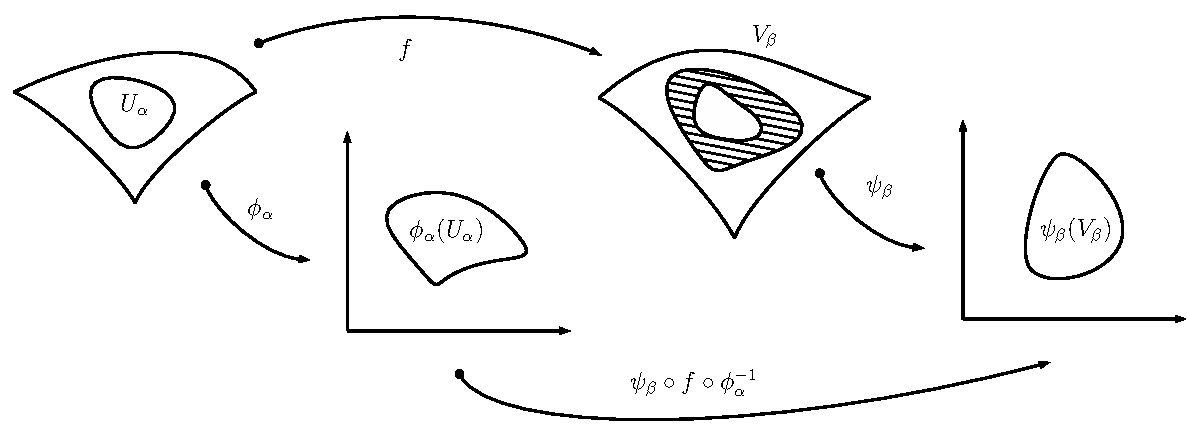
\includegraphics[width=13cm]{figura2.pdf}}
%
 \leyenda{Cartas  coordenadas  usadas  en   la  definici\'on  de  una  funci\'on
   diferenciable.}
\end{figure}

Cualquier  superficie ``suave''  en $\Rset^3$  es un  ejemplo de  (sub) variedad
diferenciable. Este ejemplo no debe conducir  a la confusi\'on de pensar que una
variedad debe estar inmersa en $\Rset^n$. Otro ejemplo de variedad diferenciable
de dimensi\'on $n$ es la esfera $\Sset^n$, definida previamente.

\begin{definicion}[Diferenciabilidad de clase $C^k$]
  Dadas  dos variedades  $\M$ y  $\M'$ de  clase $C^r$,  una  aplicaci\'on $f:\M
  \rightarrow \M' $,  se dice {\it diferenciable} de clase $C^k,  \quad k \le r$
  si para  toda carta  $\left( U_\alpha  , \phi_\alpha \right)$  de $\M$  y toda
  carta  de $\left(  V_\beta ,  \psi_\beta \right)$  de $\M'$  tal  que $f\left(
    U_\alpha \right) \subset V_\beta$, la aplicaci\'on $\psi_\beta \circ f \circ
  \phi_\alpha^{-1}$ de $\phi_\alpha\left( U_\alpha \right)$ en $\psi_\beta\left(
    V_\beta \right)$, es diferenciable de clase $C^k$.
\end{definicion}

El disponer  de la noci\'on de  funci\'on diferenciable, permite  asignar a cada
punto de una variedad diferenciable,  un espacio vectorial. \'Este estar\'a dado
por operadores  lineales que act\'uan  sobre funciones diferenciables y  dan por
resultado un n\'umero.  Antes de ir a la definici\'on  de ese espacio vectorial,
introducimos el concepto de curva suave sobre una variedad.
%
\begin{definicion}[Curva de clase $C^k$ sobre una variedad]
  Sea $\M$  una variedad de  clase $C^r$. Una  curva $\lambda$ en $\M$  de clase
  $C^k, \quad k  \le r$ es una funci\'on  del intervalo real $[a \, ,  \, b]$ en
  $\M$ tal que  para toda carta $\left( U_\alpha ,  \phi_\alpha \right)$ en $\M$
  la composici\'on
  %
  \[
  \phi_\alpha \circ \gamma: [a \, , \, b] \rightarrow \phi_\alpha\left( U_\alpha
  \right)
  \]
  %
  es de clase $C^k$. En coordenadas
  %
  \[
  \phi_\alpha \circ \gamma (t) = \{ x^1(t) , \ldots , x^n(t) \}
  \]
\end{definicion}
%
Con esto podemos ahora dar la noci\'on de vector tangente a una variedad:
%
\begin{definicion}[Tangente a una variedad]
  Sea $\F(p)$ el  conjunto de funciones diferenciables de  clase $C^1$ definidas
  en un entorno del punto $p$.  Sea $\gamma(t)$ una curva de clase $C^1$, $a \le
  t  \le b$  tal que  $\gamma(t_0) =  p$. El  vector {\it  tangente} a  la curva
  $\gamma(t)$ en el punto $p$ es una aplicaci\'on $\mathbb{X}_p : \F(p) \rightarrow \Rset$
  % \[
  % \mathbb{X}_p : \F(p) \rightarrow \Rset
  % \]
  cuyo efecto es
  %
  \[
  \mathbb{X}_p f = \frac{df(\gamma (t))}{dt} |_{t_0}
  \]
\end{definicion}
%
El vector $\mathbb{X}_p$ satisface las siguientes propiedades
%
\begin{itemize}
 \item $\mathbb{X}_p$ es una aplicaci\'on lineal de $\F(p)$ en $\Rset$,
  %
 \item  $\mathbb{X}_p(fg) =  \left( \mathbb{X}_p  f \right)  g(p) +  f(p) \left(
     \mathbb{X}_p g \right)$ para $f , g \in \F(p)$.
\end{itemize}
%
Dejamos para el lector demostrar estas propiedades.

Sean $(u^1 , \ldots  , u^n)$ coordenadas locales en un entorno  $U$ de $p$. Para
cada $j$, $\left( \frac{\partial}{\partial  u^j} \right)|_p$ es una aplicaci\'on
de $\F(p)$  en $\Rset$ la cual satisface  las propiedades (i) e  (ii). Veremos a
continuaci\'on que el conjunto de todas las aplicaciones $\mathbb{X}$ de $\F(p)$
en $\Rset$ es un espacio vectorial $n$-dimensional, siendo $n$ la dimensi\'on de
la variedad diferenciable $\M$.

Dada una  curva $\gamma(t)$ con $\gamma(t_0)  = p$, sean  $u^j(t) = \gamma^j(t),
\quad  j =  1 ,  \ldots ,  n$  las coordenadas  locales de  esa curva.  Entonces
$\frac{df(\gamma(t))}{dt}|_{t_0}  =  \sum_j  \left(  \frac{\partial  f}{\partial
    u^j}|_p  \right)  \left( \frac{d  \gamma^j  (t)}{dt} \right)|_{t_0}$.  Extra %% ESTA???
expresi\'on indica  que todo vector  en $p$ es  una combinaci\'on lineal  de los
vectores (operadores).

\begin{equation}
\left(\frac{\partial}{\partial u^1}|_p \right),\ldots,\left(\frac{\partial}{\partial u^n}|_p \right) \label{set}
\end{equation}

Sea la  combinaci\'on lineal  $\sum_j \xi^j \frac{\partial}{\partial  u^j}|_p$ y
sea la curva definida por
%
\[
u^j(t) = u^j(p) + \xi^j t \quad j = 1 , \ldots , n
\]
%
El   vector   tangente   a   esta   curva   en  $t   =   0$   es   $\sum   \xi^j
\frac{\partial}{\partial u^j}|_p$.  Adem\'as si
%
\[
\sum \xi^j \frac{\partial}{\partial u^j}|_p =0,
\]
%
entonces
%
\[
0 = \sum \xi^j \left( \frac{\partial u^k}{\partial u^j} \right)|_p = \xi^k \quad
k = 1 , \ldots , n
\]
%
Esto demuestra la independencia lineal de los vectores~\eqref{set}.
%
\begin{definicion}[Espacio tangente]
  El conjunto  de vectores tangentes en $p  \in \M$, es llamado  el {\it espacio
    tangente de $\M$ en $p$}, y lo denotaremos por $T_p(\M)$.
\end{definicion}

La colecci\'on de todos los  espacios tangentes, $\bigcup_{p \in \M} T_p(\M)$ se
llama {\it fibrado tangente}.

Al fibrado tangente se le puede  dar la estructura de un \'algebra (\'algebra de
Lie). Esta surge de calcular  el conmutador $[\mathbb{X}, \mathbb{Y}]$ entre dos
campos vectoriales $\mathbb{X}$ e $\mathbb{Y}$:
%
\[
[\mathbb{X},  \mathbb{Y}] f  \equiv  \left( \mathbb{X}  \mathbb{Y} -  \mathbb{Y}
  \mathbb{X} \right) f
\]
%
Si los vectores  se escriben en t\'ermino de los vectores  de la base coordenada
$\left(  \frac{\partial}{\partial  x^a}  \right)$,  el  conmutador  entre  ellos
resulta ser el vector:
%
\[
\sum_{ab} X^a \frac{\partial  Y^b}{\partial x^a} \frac{\partial}{\partial x^b} -
\sum_{ab} Y^a \frac{\partial X^b}{\partial x^a} \frac{\partial}{\partial x^b}
\]

A cada espacio tangente $T_p(\M)$ podemos asignar su dual, $T_p^*(\M)$, es decir
el conjunto de  todos los operadores lineales y  homog\'eneos que act\'uan sobre
$T_p(\M)$.   A    un   elemento   del   espacio   dual    lo   llamaremos   {\it
  $1$-forma}. Denotaremos a  la acci\'on de un elemento  de $T_p^*(\M)$, digamos
$\omega_p$, por:
%
\[
\omega_p(\mathbb{X}_p) = \left\langle \omega_p , \mathbb{X}_p \right\rangle.
\]
%
Para cada  funci\'on $f \in  \F(p)$, el {\it  diferencial de $f$},  denotado por
$(df)_p$, es el elemento de $T_p^*(\M)$ que tiene por acci\'on:
%
\[
\left\langle (df)_p ,  \mathbb{X}_p \right\rangle = \mathbb{X}_p f,  \quad \mathbb{X}_p \in
T_p(\M)
\]

Cada funci\'on coordenada $u^j$ es una funci\'on de $\M$ sobre $\Rset$. Entonces
podemos  calcular  el  diferencial  de  $u^j$, cuya  acci\'on  sobre  un  vector
$\mathbb{X}_p \in T_p(\M)$ est\'a dada por
%
\[
 \left\langle (du^j)_p , \mathbb{X}_p \right\rangle = \mathbb{X}_p^j
\]
%
En particular,  si $\mathbb{X}_p =  \left(\frac{\partial}{\partial u^k} \right)$
resulta
%
\[
\left\langle   (du^j)_p   ,   \left(   \frac{\partial}{\partial   u^k}   \right)
\right\rangle = \delta_k^j;
 \]
%
 es decir $\left\{ (du^j)_p \right\}_{j=1}^n$ es la base dual de $\left\{ \left(
     \frac{\partial}{\partial  u^j} \right)_p \right\}_{j=1}^n$.  Toda $1$-forma
 $\omega$ se puede escribir en t\'ermino de esta base:
%
\[
\omega = \sum_a \omega_a dx^a
\]

Con los espacios  $T_p(\M)$ y $T_p^*(\M)$ podemos construir  el espacio producto
cartesiano
%
\[
\left(  T_p(\M)  \right)_s^r =  T_p(\M)  \times  T_p(\M)  \ldots T_p(\M)  \times
T_p^*(\M) \times T_p^*(\M) \ldots \times T_p^*(\M)
\]
%
con $r$ factores de $T_p(\M)$ y $s$ factores de $T_p^*(\M)$.

\begin{definicion}[Tensor de tipo $(r,s)$]
  Un {\it tensor de tipo $(r,s)$} es un operador $S$,
  %
  \[
  S: \left( T_p(\M) \right)_s^r \rightarrow \Rset
  \]
  %
  que es lineal y homog\'eneo en cada uno de sus argumentos.
\end{definicion}

\begin{definicion}[Campo tensorial]
  Un {\it campo tensorial $S$ de  clase $C^k$ de tipo $(r,s)$ sobre $V \subseteq
    \M$} es un mapa  $C^k$ que asigna un tensor de tipo  $(r,s)$ a cada punto $p
  \in V$.
\end{definicion}
%
En  t\'ermino  de las  bases  $\left\{  \left( \frac{\partial}{\partial  u^j}|_p
  \right)  \right\}_{j=1}^n$  y $\left\{  (du^j)_p  \right\}_{j=1}^n$, el  campo
tensorial $S$ se puede escribir:
%
\[
S(p) = S^{a_1 \ldots  a_r}_{b_1 \ldots b_s}(p) \frac{\partial}{\partial x^{a_1}}
\bigotimes   \ldots  \bigotimes  \frac{\partial}{\partial   x^{a_r}}  \bigotimes
dx^{b_1} \bigotimes \ldots \bigotimes dx^{b_s}
\]
%
\noindent donde  las funciones $S^{a_1 \ldots a_r}_{b_1 \ldots b_s}$  son de clase
$C^k$ y $\bigotimes$ es el producto tensorial.

Entre los campos tensoriales que se  pueden definir sobre una variedad $\M$, hay
uno particularmente importante,  y es conocido como el  tensor m\'etrico. \'Este
se define por medio de un producto escalar:
%
\begin{definicion}[Producto escalar]
  Un {\bf producto escalar} sobre $T_p(\M)$ es una funci\'on
  %
  \[
  g: T_p(\M) \times T_p(\M) \rightarrow \Rset
  \]
  %
  que satisface
  %
  \begin{enumerate}
  \item $g(\mathbb{X}, \mathbb{Y}) = g(\mathbb{Y}, \mathbb{X}), \quad \text{para}
    \quad \mathbb{X}, \mathbb{Y} \in T_p(\M)$
  %
  \item  $g(\mathbb{X},   a  \mathbb{Y}  +  b  \mathbb{Z})   =  a  g(\mathbb{X},
    \mathbb{Y}) + b g(\mathbb{X}, \mathbb{Z})$
  \end{enumerate}
\end{definicion}

El producto escalar se dice  {\it no degenerado} si $g(\mathbb{X}, \mathbb{Y})=0
\quad \forall \:  \mathbb{Y} \in T_p(\M)$ implica $\mathbb{X}  = 0$.  Obviamente
el  producto  escalar  es un  tensor  de  tipo  $(0,2)$.  Como  campo  tensorial
$g(\;,\;)$   se   puede   expresar    en   t\'erminos   de   la   base   $\left(
  \frac{\partial}{\partial    u^1}|_p     \right)    ,    \ldots     ,    \left(
  \frac{\partial}{\partial u^n}|_p \right)$
%
\[
g(\mathbb{X}, \mathbb{Y})  = \sum_{ab} X^a  Y^b g\left( \frac{\partial}{\partial
    u^a}, \frac{\partial}{\partial u^b} \right)
\]
%
o, de manera equivalente
%
\[
g(\mathbb{X}, \mathbb{Y}) = \sum_{ab} g_{ab} X^a Y^b
\]
%
donde     $g_{ab}    =    g     \left(    \frac{\partial}{\partial     u^a}    ,
  \frac{\partial}{\partial  u^b}   \right)$.  Si  el  producto   escalar  es  no
degenerado, entonces  existe la  matriz inversa de  la matriz $g_{ab}$,  a cuyos
elementos los denotaremos por $g^{ab}$, de modo que
%
\[
\sum_c g_{ac} g^{cb} = \delta_a^b
\]

La  existencia de  un campo  tensorial  m\'etrico (o  producto escalar  definido
localmente),  permite introducir  la idea  de {\it  longitud de  una  curva}. En
efecto, sea  $\gamma(t), \quad t  \in [a \,  , \, b]$  una curva de  clase $C^1$
sobre $\M$,  que une los  puntos $p$  y $q$: $\gamma(a)  = p, \quad  \gamma(b) =
q$. En el punto $\gamma(t)$ tenemos  el vector tangente a la curva $\gamma$ dado
por
%
\[
\left( \frac{\partial}{\partial t} \right)_\gamma = \sum_j \frac{d \gamma^j}{dt}
\frac{\partial}{\partial x^j}
\]

\begin{definicion}[Longitud de una curva]
  La {\it longitud de la curva $\gamma$  entre los puntos $p$ y $q$} est\'a dada
  por la cantidad
  %
  \begin{equation}
    L = \int_a^b | g \left( \frac{\partial}{\partial t}, \frac{\partial}{\partial t} \right) |^{\frac{1}{2}} dt
  \label{longitud}
  \end{equation}
\end{definicion}
%
O, equivalentemente
%
\begin{equation}
L = \int_a^b \left| \sum_{ij} g_{ij}(x) \frac{d\gamma^i}{dt} \frac{d \gamma^j
}{dt} \right|^{\frac{1}{2}} dt \label{longitud}
\end{equation}

% ============================== Estructura Afin ============================= %

%\sub
\seccion{Estructura Afin}
\label{s:WL:EstructuraAfin}

En  el espacio  eucl\'ideo  $n$-dimensional (pensado  aqu\'i  como una  variedad
diferenciable),  cuando  usamos coordenadas  cartesianas,  caracterizamos a  dos
vectors paralelos como aquellos  que tienen iguales componentes. Si reemplazamos
las coordenadas cartesianas por las polares, por ejemplo, esta caracterizaci\'on
deja  de  ser  v\'alida.  Veamos   c\'omo  podemos  introducir  la  noci\'on  de
paralelismo de vectores, usando  cualquier sistema de coordenadas. Sea $\{x^a\}$
el sistema de  coordenadas cartesiano del espacio. En  este sistema, hemos dicho
que  dos vectores  paralelos,  por ejemplo  $\mathbb{V}$ y  $\tilde{\mathbb{V}}$
tienen iguales componentes:
%
\[
V^a = \tilde{V}^a
\]
%
Si el vector $\mathbb{V}$ es tangente al espacio en el punto $p$ con coordenadas
$\{ x^a \}$  y el vector paralelo $\tilde{\mathbb{V}}$ es  tangente al punto $q$
con coordenadas ${x^a+\delta x^a}$, vale
%
\[
\tilde{V}^a(q)-V^a(p) = 0
\]
%
Dado  un  vector $\mathbb{V}$  en  $p$, podemos  definir  un  campo de  vectores
paralelos  a $\mathbb{V}$  en un  entorno  de $p$.  Denotemos a  este campo  por
$\tilde{\mathbb{V}}$.  Este  campo cumple  que  en  el  punto $p$  coincide  con
$\mathbb{V}$ y con la condici\'on:
%
\[
\tilde{V}^a(x+\delta x) -  V^a(x) = \frac{\partial \tilde{V}^a}{\partial x^b}(p)
\delta x^b
\]
%
Sea ${\xi^a}$ otro sistema de  coordenadas para el espacio eucl\'ideo, vinculado
con ${x^a}$ mediante las relaciones
%
\begin{equation}
\xi^a = \xi^a(x^b), \quad x^b=x^b(\xi^a) \label{cambcoor}
\end{equation}
%
A partir de ellas, resulta
%
\begin{equation}
\delta \xi^a = \frac{\partial \xi^a}{\partial x^b} \delta x^b, \qquad \delta x^b = \frac{\partial x^b}{\partial \xi^a} \delta \xi^a
\end{equation}
%
Las componentes de $\tilde{\mathbb{V}}$ se transforman de acuerdo con
%
\[
\tilde{V}^a = \frac{\partial x^a}{\partial \xi^b} \tilde{V'}^b
\]
%
donde  $\tilde{V'}^a$  son  las   componentes  de  $\tilde{\mathbb{V}}$  en  las
coordenadas $\{\xi^a\}$. Entonces, podemos escribir
%
\begin{eqnarray}
\frac{\partial \tilde{V}^a}{\partial x^b} &=& \frac{\partial}{\partial \xi^c} \left(\frac{\partial x^a}{\partial \xi^d} \tilde{V'}^d \right) \frac{\partial \xi^c}{\partial x^b}  \nonumber \\
%
& = & \frac{\partial^2 x^a}{\partial \xi^c \partial \xi^d} \tilde{V'}^d \frac{\partial \xi^c}{\partial x^a}+ \frac{\partial x^a}{\partial \xi^d} \frac{\partial{\tilde{V'}^d}}{\partial \xi^c} \frac{\partial \xi^c}{\partial x^b}
\end{eqnarray}
%
Si    definimos   la    cantidad   $\delta    \tilde{V'}^d    =   \frac{\partial
  \tilde{V'}^d}{\partial x^e} \delta \xi^e$ y despu\'es de un poco de \'algebra,
llegamos a la relaci\'on
%
\begin{equation}
\delta \tilde{V'}^n = - \frac{\partial^2 x^a}{\partial \xi^e \partial \xi^d} \frac{\partial \xi^n}{\partial x^a} \tilde{V'}^d \delta \xi^e \label{con}
\end{equation}
%
Esta expresi\'on puede reescribirse de la siguiente forma:
%
\begin{equation}
\delta \tilde{V'}^n = - \Gamma'^n_{ed} \tilde{V'}^d \delta \xi^e
\end{equation}
%
\noindent  en   donde  los  coeficientes  $\Gamma'$  est\'an   definidos  en  la
expresi\'on~\eqref{con}. De su definici\'on resulta que las cantidades $\Gamma'$
se anulan para cambios {\it lineales} de coordenadas~\eqref{cambcoor}.

Obs\'ervese que al haber arribado a la definici\'on de los coeficientes $\Gamma$
no hemos hecho uso de ninguna  propiedad especial del espacio eucl\'ideo. Es por
ello  que  la  expresi\'on~\eqref{con}   es  v\'alida  para  cualquier  variedad
n-dimensional. Es f\'acil ver que frente a un cambio de coordenadas
%
\begin{equation}
x^a \rightarrow x'^a= x'^a\left(x^b\right) \label{camb2}
\end{equation}
%
las cantidades $\Gamma$ cambian seg\'un la expresi\'on
%
\begin{equation}
\Gamma ^f_{de} = \Gamma'^a_{mn} \frac{\partial x^f}{\partial x'^a} \frac{\partial x'^m}{\partial x^d} \frac{\partial x'^n}{\partial x^e}+\frac{\partial x^f}{\partial x'^a} \frac{\partial^2 x'^a}{\partial x^e \partial x^d} \label{camcon}
\end{equation}
%
Debemos  remarcar que  esta  ley  de transformaci\'on  es  lineal y  homog\'enea
(tensorial)   s\'olo  cuando  el   cambio  de   coordenadas~\eqref{cambcoor}  es
lineal. Esta propiedad  de los coeficientes $\Gamma$ nos  permite generalizar la
idea de paralelismo en una variedad arbitraria:
%
\begin{definicion}[Conexi\'on af\'in]
  Cuando  en una  variedad  n-dimensional arbitraria  $\M$  se introducen  $n^3$
  coeficientes $\Gamma$ que se transforman de acuerdo con la ley~\eqref{camcon},
  diremos que sobre esa variedad se ha definido una {\it conexi\'on af\'in}
\end{definicion}

A partir de los coeficientes $\Gamma$ es posible definir una nueva derivada para
un campo vectorial arbitrario, digamos $V^a(x)$:
%
\begin{definicion}[Derivada covariante de campo]
  Sea  un campo vectorial  $V$ definido  en un  entorno del  punto $x$.  La {\it
    derivada covariante  del campo  $V$} est\'a dado  por las componentes  de un
  tensor de tipo $(1,1)$
  %
  \[
  V^a_{;c} = V^a_{,c} + \Gamma^a_{bc} V^b
  \]
\end{definicion}

\begin{definicion}[Derivada covariante en una direcci\'on]
  Dados dos campos  vectoriales $U(x)$ y $V(x)$, la  {\it derivada covariante de
    $V$ en la direcci\'on de $U$} es el campo vectorial definido por
  %
  \[
  U(x) \cdot \nabla V(x) \equiv \sum_{ab} V^a_{;b}(x) U^b(x) \mathbb{E}_a \equiv
  \nabla_U V
  \]
% hdot => cdot?
\end{definicion}
%
donde  $\mathbb{E}^a$ es  el campo  de  vectores coordenados  asociados con  las
coordenadas $x^a$. Esta \'ultima  definici\'on permite trasladar paralelamente a
un vector a  lo largo de una  curva. Basta con tomar como  $\mathbb{U}$ al campo
tangente a la curva.


% ============================== Variedad Riemanniana ============================= %

%\sub
\seccion{Variedad Riemmanniana}
\label{s:WL:VariedadRiemmanniana}

Sea $\M$ una variedad diferenciable  $n$-dimensional. Si $\M$ tiene definida una
m\'etrica  no   singular  sobre  ella,   recibe  el  nombre  de   {\it  variedad
  Riemanniana}. La existencia de una m\'etrica sobre $\M$ permite introducir una
conexi\'on af\'in  particular, conocida como la conexi\'on  de Levi-Civita. Sean
$g_{ab}$ y  $g^{ab}$ los coeficientes de la  m\'etrica $g$ y su  inversa, en las
coordenadas $\{x^a\}$, respectivamente.

Para  dos puntos  pr\'oximos,  la separaci\'on  entre  ellos viene  dada por  la
expresi\'on:
%
\begin{equation}
ds^2 = \sum_{ab} g_{ab} dx^a dx^b \label{quad}
\end{equation}

Adem\'as de definir una distancia  entre puntos pr\'oximos, la existencia de una
m\'etrica  permite   definir  una  conexi\'on  particular   sobre  una  variedad
riemanniana:
%
\begin{definicion}[Conexi\'on de Levi-Civita]
  La conexi\'on de Levi-Civita en las coordenadas $x^a$ est\'a dada por:
  %
  \begin{equation}
  \Gamma^a_{bc} = \frac{1}{2} \sum_d g^{ad} \left(g_{bd,c} + g_{cd.b} - g_{bc.d} \right) \label{levi}
  \end{equation}
\end{definicion}

La existencia  de esta  particular conexi\'on no  imposibilita la  existencia de
otras conexiones definidas sobre $\M$.

Como hemos visto  m\'as arriba, el tener definida  una m\'etrica permite definir
la  longitud de  una curva.  Bajo ciertas  condiciones, que  supondremos  que se
satisfacen, podemos plantearnos el problema  de determinar la curva que minimiza
(en  realidad  extremiza)  su  longitud  al  unir  dos  puntos  fijos  sobre  la
variedad. Esto se puede tratar  resolviendo el problema variacional asociado con
el funcional~\eqref{longitud}. La ecuaci\'on de Euler-Lagrange  conduce en este
caso a:
%
\begin{equation}
\frac{d^2 x^d}{dt^2} + \Gamma^d_{ca} \frac{dx^c}{dt} \frac{dx^a}{dt} = 0 \label{geode}
\end{equation}
%
\noindent donde $x^a(t)$ son las coordenadas de la curva y $t$ es un par\'ametro
adecuadamente elegido. Una curva  que satisface~\eqref{geode}, se llama una {\it
  curva geod\'esica}.  Es posible caracterizar  a una curva geod\'esica  de otro
modo. Sea  $\mathbb{U}(t)$ el vector  tangente a una curva  $\gamma(t)$ definida
sobre $\M$.  La curva $\gamma$ se  dice una geod\'esica si su vector tangente es
trasladado paralelamente a lo largo de ella:
%
\[
\mathbb{U} \cdot \nabla \mathbb{U} = f(t) \mathbb{U}
\]
% 
% hdot => cdot?
Siempre es posible  elegir al par\'ametro $t$ de forma tal  que $f(t)=0$, con lo
cual reobtenemos la ecuaci\'on~\eqref{geode}.

El disponer de geod\'esicas, permite dar a una variedad riemanniana el car\'cter
de espacio m\'etrico.  En efecto, podemos definir la  distancia entre dos puntos
$p$ y $q$ de la variedad $\M$ a trav\'es de la expresi\'on:
%
\begin{equation}
d(p,q) = \min_{\gamma} L(\gamma) \label{distt}
\end{equation}
%
\noindent donde  el m\'inimo  se eval\'ua  entre todas las  curvas que  unen los
puntos $p$ y $q$, y $L$ es la longitud~\eqref{longitud}. Como siempre, todo esto
es  posible ser  realizado  localmente.   Las geod\'esicas  son  las curvas  que
localmente  minimizan  la distancia  entre  dos  puntos.  La distancia  definida
por~\eqref{distt}  verifica  la  desigualdad   triangular,  y  por  eso  es  una
m\'etrica.

Dada una conexi\'on  $\nabla$ se define un tensor de  tipo $(1,3)$, llamado {\it
  tensor de curvatura} asociado a la conexi\'on $\nabla$, cuya espresi\'on es:
%
\[
\R\left( \mathbb{X} , \mathbb{Y} \right) \mathbb{Z} = \nabla_{\mathbb{X}} \left(
  \nabla_{\mathbb{Y}}   \mathbb{Z}    \right)   -   \nabla_{\mathbb{Y}}   \left(
  \nabla_{\mathbb{X}}  \mathbb{Z}   \right)  -  \nabla_{[\mathbb{X},\mathbb{Y}]}
\mathbb{Z}
\]
%
Si los  vectores $\mathbb{X}$, $\mathbb{Y}$ y $\mathbb{Z}$  son reemplazados por
los       vectors       coordenados       $\frac{\partial}{\partial       x^a}$,
$\frac{\partial}{\partial     x^b}$    y     $\frac{\partial}{\partial    x^c}$,
respectivamente, resulta
%
\[
\R\left( \frac{\partial}{\partial  x^a} , \frac{\partial}{\partial  x^b} \right)
\frac{\partial}{\partial x^c} = R^d_{cab} \frac{\partial}{\partial x^d}
\]
%
con
%
\[
R^d_{cba}   \equiv  \left(  \frac{   \partial  \Gamma^d_{cb}}{\partial   x^a}  +
  \Gamma^d_{ra} \Gamma^r_{cb}  - \frac{ \partial  \Gamma^d_{ca}}{\partial x^b} -
  \Gamma^d_{rb} \Gamma^r_{ca}\right) \frac{\partial}{\partial x^d}
\]

{\bf  Nota:} Si  bien existe  una motivaci\'on  geom\'etrica para  introducir el
tensor de curvatura, aqu\'i no la hemos  dado. Ella tiene que ver con la idea de
cu\'anto cambia un  vector al desplazarlo paralelamente a lo  largo de una curva
cerrada. En general diremos que una  variedad es plana, si todas las componentes
de su tensor de curvatura, se anulan.

Concluimos  este cap\'itulo  con una  breve  nota hist\'orica.  En sus  trabajos
originales sobre geometr\'ia, B. Riemann  introdujo el elemento de l\'inea entre
dos puntos vecinos $p$ y $q$ por medio de la expresi\'on
\begin{equation}
ds = F(p, \mathbb{X})dt \label{linea}
\end{equation}
%
con $F(  p , \mathbb{X} )$  una funci\'on homog\'enea  de grado 2 en  la segunda
variable. Aqu\'i estamos suponiendo que  los puntos $p$ y $q$ tienen coordenadas
${x^a}$  y ${x^a +  X^a dt}$,  respectivamente. La  geometr\'ia basada  sobre el
elemento de l\'inea  se conoce como geometr\'ia de  Finsler.  Obs\'ervese que el
elemento~\eqref{quad} (de  Riemann) es un  caso particular de la  geometr\'ia de
Finsler.

